% Draft manuscript. Written by an AI assistant (Claude) for the researcher to edit.
% Real-data results are PLACEHOLDERS until the pre-registration is approved and the
% gated pipeline has run. Every number in this file is listed with its source in
% paper/notes.md. Compile: pdflatex main && bibtex main && pdflatex main && pdflatex main
\documentclass[11pt,a4paper]{article}
\usepackage[utf8]{inputenc}
\usepackage[T1]{fontenc}
\usepackage[margin=2.5cm]{geometry}
\usepackage{amsmath}
\usepackage{booktabs}
\usepackage{graphicx}
\usepackage[round,authoryear]{natbib}
\usepackage{xcolor}
\usepackage[hidelinks]{hyperref}

% Placeholder for anything that needs the real data or a decision by the researcher.
\newcommand{\TBD}[1]{\textcolor{red}{[TBD: #1]}}

\title{Is alpha really missing? A pre-registered spectral parameterization of resting EEG
in adults from India and Tanzania, with a simulation test of the detection method}
\author{[AUTHORS --- TBD]}
\date{Draft of 25 November 2026. Real-data results are not yet computed.}

\begin{document}
\maketitle

\begin{abstract}
\noindent
The alpha rhythm is usually treated as a universal feature of the resting human
electroencephalogram (EEG), yet a 2017 preprint reported that it is ``largely undetected''
in Indian adults without post-primary education or access to modern technologies. That
study did not model the aperiodic ($1/f$-like) background of the spectrum, which can make
a peak look weak or absent. We reanalyse an open dataset of resting EEG from 1,000
participants in India and 1,000 in Tanzania (OpenNeuro ds007358) with spectral
parameterization (specparam). The analysis plan was written before any spectrum of the
real recordings was computed. Before running it, we tested the full pipeline on simulated
recordings with known ground truth at the headset's 128~Hz sampling rate.
\textbf{Simulation results:} with common settings (minimum peak height 0.1 $\log_{10}$
units), specparam reported an alpha peak in 73--83\% of simulated recordings that contained
no alpha, at every recording length from 30 to 180~s. Requiring a fitted peak height of at
least 0.25 reduced this to 4\% for 60~s recordings and to 0\% for longer ones, while peaks
of true height 0.3 or more were still found in 98--100\% of recordings; weaker peaks could
not be separated from chance.
\textbf{Real-data results:} \TBD{presence rate per site with 95\% CI (H1); quality and
income as predictors of a missing peak (H2); age slopes of alpha frequency, aperiodic
exponent and alpha power (H3--H5); one sentence on meaning}. Differences between the two
sites are described as differences in environment, recording context and data quality,
not as traits of any population.
\end{abstract}

% ---------------------------------------------------------------------------
\section{Introduction}

The alpha rhythm, an oscillation of about 8--12~Hz that is strongest over posterior scalp
when the eyes are closed, is the most prominent feature of the resting human EEG
\citep{klimesch1999}. Two of its properties change across adulthood. The individual alpha
frequency (IAF) slows in older age \citep{klimesch1999,cesnaite2023,merkin2023}. The
aperiodic background of the spectrum, which falls off roughly as $1/f^{\chi}$, becomes
flatter: the exponent $\chi$ is lower in older than in younger adults
\citep{voytek2015,donoghue2020}.

Almost all of this knowledge comes from samples in Western, educated, industrialised, rich
and democratic societies, which are a narrow and unusual slice of humanity
\citep{henrich2010}. Multinational EEG norms exist \citep{li2022}, but they pool sites that
used different recording systems, so differences between countries cannot be separated
from differences between devices.

Against this background, \citet{parameshwaran2017} reported a striking result from 402
adults in 48 settlements in Tamil Nadu, India, recorded with a 14-channel Emotiv EPOC
headset. Alpha was ``largely undetected in the EEG of adults without post-primary
education and access to modern technologies''. In their data, 20\% of participants showed
no oscillation in any channel, and only 40\% of the ``pre-modern and transitioning''
groups had alpha energy above the noise level, against 93.3\% of the ``modern'' group. The
authors themselves described ``a very broad continuum rather than an absolute absence''.
The preprint has not appeared in a journal. A later study of 1,199 adults in rural
Haryana, India, with the same headset model found an alpha peak in 71.3\% of eyes-closed
recordings \citep{bhavnani2022}. By comparison, an automated method found a peak
frequency in 61 of 63 healthy adults (97\%)
\citep{corcoran2018}.

These studies share a limitation. None of them fitted a model of the aperiodic background.
\citet{parameshwaran2017} located peaks with the second derivative of the power spectrum,
and \citet{bhavnani2022} describe the peak only as activity ``above the background
envelope'' of the spectrum. This matters because the height of a spectral peak is measured
against its background. If the background is steeper, flatter or noisier in one group of
recordings than in another (because of age, electrode contact, movement or line noise),
the same oscillation can look strong, weak or absent
\citep{donoghue2020,donoghue2022,gerster2022}. In European samples, much of the apparent
decline of alpha \emph{power} with age is explained by the change in the aperiodic
background. After adjusting for it, \citet{merkin2023} and \citet{cesnaite2023} found no
reliable age difference in alpha power, while \citet{trondle2023} found that the age
effect was overestimated by conventional analyses but did not vanish. A claim that alpha
is weak or missing in some group therefore needs an explicit model of the background, and
a check that ``missing'' does not simply follow recording quality.

A new open dataset makes this test possible. \citet{vianney2025} describe a field
programme that recorded resting EEG from 7,933 people in India and Tanzania with one
headset model and one protocol, operated by trained non-specialist field researchers. A
subset of 2,000 participants, 1,000 per country, is public \citep{openneuro_ds007358}.
\citet{vianney2025} focus on data quality. They also report that the frequency of the
largest spectral value in 7--12~Hz falls with age in both countries, but this measure
takes the maximum in a band and does not test whether a peak exists.

Here we apply spectral parameterization \citep[specparam;][]{donoghue2020} to the
eyes-closed and eyes-open recordings of the adults in this dataset. We ask two questions.
First, once the aperiodic background is modelled, how often is an eyes-closed occipital
alpha peak present, and where it is not detected, is this better explained by recording
quality than by income? Second, within each country, how do IAF, alpha power above the
background and the aperiodic exponent vary with age? Our hypotheses (H1--H5 and a validity
check V1; Table~\ref{tab:hyp}) were fixed in a pre-registration before any spectrum of the
real recordings was computed.

A detection method can only answer the first question if its own error rates are known. A
peak-finding algorithm applied to a noisy spectrum will sometimes report a peak where
there is none, and miss one that is there, and both errors depend on how long the
recording is and on the settings used. We therefore begin with a simulation study: we
generate recordings with a known aperiodic background and a known alpha peak (or none), at
the headset's sampling rate and at the recording lengths in the dataset, and pass them
through exactly the code used for the real data. The simulation results are reported in
full in this draft (Section~\ref{sec:simresults}). The real-data results are marked as
placeholders.

All comparisons between India and Tanzania in this paper are descriptive. The two sites
differ in electrode layouts, field teams, settings and age mix. Differences between them
are differences in environment, recording context and data quality, and we do not
interpret them as traits of any population.

% ---------------------------------------------------------------------------
\section{Data}

\subsection{Dataset}

We use OpenNeuro dataset ds007358, version 1.0.0, released on 4 February 2026 under a CC0
licence \citep{openneuro_ds007358}. It holds recordings from 2,000 participants, 1,000 in
India and 1,000 in Tanzania, in three conditions: eyes closed, eyes open, and a Raven's
matrices task. We use the first two. The participant table gives the site, an age group
(the exact age is not released), an income bin, a mental-health score and sex. There is no
education variable. How the 2,000 were drawn from the full cohort is not documented.

According to \citet{vianney2025}, recordings were made with the wireless Emotiv FLEX~2 Gel
headset, using 16 of its 32 electrode positions and an ear-clip reference, for 3~minutes
with eyes closed and 3~minutes with eyes open. Twelve field researchers were recruited in
each country, were new to EEG, and received two weeks of training. All participants gave
written informed consent, and the original study was approved by ethics committees in
India and Tanzania \citep{vianney2025}. The present work is a secondary analysis of
de-identified public data.

The public files differ from that description in two ways that matter for analysis.
First, the files are sampled at 128~Hz (256~Hz for 7 Indian participants), whereas the
paper states 256~Hz. Second, electrode layouts vary. Among the 1,000 Indian participants
there are 10 distinct layouts, although 981 share one 14-channel layout (AF3, AF4, F3, F4,
F7, F8, FC5, FC6, T7, T8, P7, P8, O1, O2). Among the 1,000 Tanzanian participants there are
136 layouts with 8 to 18 electrodes. The only posterior pair present in nearly all
recordings is O1 and O2, so this pair is our primary region. Each file also contains the
headset's own per-electrode contact-quality (CQ) and signal-quality (EQ) channels and a
flag for interpolated samples, which we use to measure recording quality.

\subsection{Participants and exclusions}

Table~\ref{tab:flow} shows the participant flow. We include adults (age groups 18--20 to
85+) whose eyes-closed recording contains both O1 and O2 and keeps at least 60~s of clean
data after epoch rejection (Section~\ref{sec:preproc}). All 225 participants under 18 are
Indian and are excluded from confirmatory analyses, as are participants without an age
group. This leaves 680 usable eyes-closed recordings in India and 786 in Tanzania. Of the
60 analysable adults excluded for too little clean data, 17 had no clean epoch at all,
because flagged samples were spread through the whole recording. The exclusion counts were
computed from time-domain quality measures only, before any spectrum existed.

\begin{table}[ht]
\centering
\caption{Participant flow. Source: \texttt{results/participants\_clean.csv} and
\texttt{results/qc\_summary.csv}. The last row is a placeholder until the fits exist.}
\label{tab:flow}
\begin{tabular}{lrr}
\toprule
 & India & Tanzania \\
\midrule
Participants in the dataset & 1,000 & 1,000 \\
Adults with a known age group & 700 & 990 \\
\quad with O1 and O2 in the eyes-closed recording & 694 & 832 \\
\quad with $\geq$ 60~s of clean eyes-closed data (usable) & 680 & 786 \\
Usable eyes-open recording as well (for V1) & 670 & 752 \\
Model fit $R^2 \geq 0.90$ (for H3--H5) & \TBD{n} & \TBD{n} \\
\bottomrule
\end{tabular}
\end{table}

The usable Indian sample is younger than the Tanzanian one: 305 of 680 Indian participants
(45\%) are aged 18--24, against 151 of 786 (19\%) in Tanzania, and only one Indian
participant is 65 or older, against 62 in Tanzania. Income is analysed in India only. In
Tanzania it is missing or in the lowest bin for almost all participants. Among the 680
usable Indian participants, income is missing for 22, and 436 of the remaining 658 fall in
the two lowest of the seven bins.

% ---------------------------------------------------------------------------
\section{Methods}

\subsection{Pre-registration and the order of work}

The hypotheses, exclusion rules, settings and models were written down in
\texttt{preregistration/prereg.md} in the project's public repository before any power
spectrum or model fit of the real recordings was computed. The scripts that compute
spectra check that this file is committed and refuse to run otherwise. \TBD{commit hash
and date of the pre-registration; list of amendments, if any}. Before the pre-registration
was fixed we had seen the participant table, the channel lists, and time-domain quality
measures for every recording (length, share of epochs kept, CQ and EQ, share of
interpolated samples, blink rate). We had also run the simulation study reported in
Section~\ref{sec:simresults}, which uses no real data. \TBD{state here which changes to
the draft pre-registration were made in response to the simulation results}.

\begin{table}[ht]
\centering
\caption{Pre-registered hypotheses and decision rules. All models are fitted separately
for each site. \TBD{update this table to the final committed pre-registration}.}
\label{tab:hyp}
\begin{tabular}{p{0.07\linewidth}p{0.45\linewidth}p{0.38\linewidth}}
\toprule
 & Hypothesis & Decision rule \\
\midrule
H1 & An eyes-closed alpha peak is present in more than 80\% of usable recordings &
Wilson 95\% CI lower bound $> 0.80$ \\
H2a & Better recording quality predicts fewer missing peaks & Logistic regression, odds
ratio $< 1$, $p < .05$ \\
H2b & In India, income has no meaningful association with a missing peak once quality is
controlled & 90\% CI of the odds ratio per SD of income rank within 0.80--1.25 \\
H3 & IAF decreases with age & Slope $< 0$, one-sided $p < .025$ \\
H4 & The aperiodic exponent decreases with age & Slope $< 0$, one-sided $p < .025$ \\
H5 & Alpha power above the background shows no meaningful change with age & 90\% CI of the
standardised slope within $\pm 0.10$ SD per decade \\
V1 & Alpha is stronger with eyes closed than with eyes open (validity check) & Share of
participants with a positive difference; Wilson 95\% CI lower bound $> 0.80$ \\
\bottomrule
\end{tabular}
\end{table}

\subsection{Preprocessing and recording quality}
\label{sec:preproc}

Recordings were processed with MNE-Python 1.10.1 \citep{gramfort2013} at their native
sampling rate. We kept the EEG electrodes and stored the headset's quality channels
separately. Signals were band-pass filtered at 1--45~Hz (zero-phase FIR) and cut into 4~s
epochs with 50\% overlap, which gives a frequency resolution of 0.25~Hz. An epoch was
rejected if it contained any sample that the headset flagged as interpolated or saturated,
or if its log-variance at O1 or O2 was more than 3 robust standard deviations above that
person's median. We use a rule relative to each person because the absolute voltages of a
consumer headset are not calibrated. A recording was usable if O1 and O2 were present and
not flat (SD of at least 1~$\mu$V) and at least 60~s were covered by accepted epochs.

In usable eyes-closed recordings the median amount of clean data was 176~s in India and
166~s in Tanzania, and the median share of epochs kept was 0.85 in both. Contact quality
at O1 and O2 was at its maximum throughout the recording in 89\% (India) and 96\%
(Tanzania) of them.

For each recording we computed five quality measures: mean EQ and mean CQ at O1 and O2,
the share of epochs kept, the share of interpolated samples, and a 50~Hz line-noise ratio
(power at 48--52~Hz divided by power at 40--45~Hz in the unfiltered signal). The quality
composite is the first principal component of these five measures after standardisation,
computed within each site and signed so that higher values mean better quality.

\subsection{Spectra}

For each accepted epoch we computed a Hann-windowed periodogram and took the median across
epochs at each frequency, a variant of Welch's method \citep{welch1967} that resists
leftover artefacts. The primary spectrum is the mean of the O1 and O2 spectra. The median
is not rescaled to the mean, so the aperiodic offset is about 0.16 $\log_{10}$ units lower
than with a mean-based estimate. This does not affect the exponent or peak heights.

\subsection{Spectral parameterization and outcome measures}

We fitted each spectrum with specparam \citep{donoghue2020}, using the \texttt{fooof}
1.1.1 implementation, over 2--40~Hz. The model describes $\log_{10}$ power as an aperiodic
line, $b - \chi \log_{10} f$ with offset $b$ and exponent $\chi$ (``fixed'' mode), plus up
to six Gaussian peaks. Peak widths were limited to 1--8~Hz, the minimum peak height was 0.1
$\log_{10}$ units above the aperiodic fit, and the peak threshold was 2 standard deviations.
The same settings were used for every recording, so that exponents are comparable.
\TBD{replace these settings with those of the final pre-registration if they change}.

Outcome measures were defined as follows. Alpha is \emph{present} if at least one fitted
peak has a centre frequency of 7--14~Hz. IAF, alpha power and alpha bandwidth are the
centre frequency, the height above the aperiodic fit, and the width of the tallest such
peak. The exponent and offset come from the aperiodic fit. Fit quality is the $R^2$ between
the model and the spectrum. A recording whose fit fails is counted as having no peak.
Alpha reactivity is the mean of the spectrum minus its aperiodic fit within IAF $\pm$ 2~Hz,
eyes closed minus eyes open, with each condition fitted separately and the window centred
on the eyes-closed IAF, or on 10.5~Hz if there is no eyes-closed peak.

As a second opinion on presence we used a simpler detector adapted from the approach of
\citet{corcoran2018}: the $\log_{10}$ spectrum is smoothed with a Savitzky--Golay filter
\citep{savitzky1964} (11 bins, order 5), and a local maximum in 7--14~Hz counts as a peak if
it rises above a straight-line fit of log power on log frequency by more than both 0.05
$\log_{10}$ units and twice the standard deviation of the residuals outside the alpha
window. This is our own implementation and not the published toolbox.

\subsection{Statistical models}

All models were fitted separately for each site with statsmodels 0.14.5
\citep{seabold2010}. Age enters as the midpoint of the age group in decades. Covariates are
sex, the quality composite, the field-researcher group as a fixed effect, and, in
Tanzania, the electrode-layout family. The field-researcher group is the letter prefix of
the participant identifier; that this prefix identifies the researcher is our assumption
and is not documented \TBD{update if the data owners confirm or correct this}.

H1 uses the proportion of usable recordings with a peak, with a Wilson confidence interval
\citep{wilson1927}. H2 uses logistic regression of a missing peak on the quality composite
and covariates, with income rank added in India. H3 to H5 use ordinary least squares with
heteroscedasticity-consistent (HC3) standard errors \citep{long2000}, on recordings with
$R^2 \geq 0.90$ (and, for IAF and alpha power, a detected peak). H1, H2 and V1 use all
usable recordings whatever the fit quality, so that poor fits cannot be removed from the
``absent'' group. The two ``no meaningful effect'' hypotheses (H2b, H5) are tested with two
one-sided tests for equivalence \citep{lakens2017}. The eleven confirmatory tests (H1, H2a,
H3, H4 and H5 in each site, and H2b in India) are corrected with Holm's method
\citep{holm1979}.

\subsection{Robustness analyses}

We report (i) a specification curve \citep{simonsohn2020} over 324 versions of the analysis
per site (three regions, three fit ranges, two aperiodic modes, six minimum peak heights
and three $R^2$ floors); (ii) refits leaving out each field-researcher group in turn;
(iii) the raw 7--12~Hz maximum used by \citet{vianney2025} next to the specparam IAF;
(iv) agreement between specparam and the second detector (Cohen's $\kappa$); (v) a null
calibration, in which aperiodic-only recordings matched to each site's fitted exponents,
offsets and recording lengths are simulated and the share with a ``detected'' peak is
reported; (vi) the models without the quality covariate; and (vii) the analysis without
the seven recordings sampled at 256~Hz.

\subsection{Simulation study}
\label{sec:simmethods}

To measure the error rates of the detection method we simulated recordings with a known
spectrum. Each simulated recording is a stationary Gaussian time series sampled at 128~Hz
whose power spectrum follows the model that specparam assumes:
\begin{equation}
\log_{10} P(f) = b - \chi \log_{10} f + h \exp\!\left(-\frac{(f - f_\alpha)^2}{2 s^2}\right),
\end{equation}
with offset $b$, exponent $\chi$, and an alpha peak of height $h$ (in $\log_{10}$ units
above the background), centre $f_\alpha$ and width $s$. Setting $h = 0$ gives a recording
with no alpha. Two channels, standing for O1 and O2, share 70\% of their variance. Each
simulated recording then passes through the same functions as the real data: the 1--45~Hz
filter, epoching and rejection, the median periodogram, and the specparam fit with the
primary settings. Because the truth is known, we can count how often a peak is reported
when none exists (a false ``present''), how often a true peak is missed (a false
``absent''), and how accurately IAF, the exponent and peak height are recovered.

Eleven experiments were run (Table~\ref{tab:simdesign}). The main experiment (A) crosses
four exponents (0.5, 1.0, 1.5, 2.0), eight alpha heights (0, 0.05, 0.1, 0.15, 0.2, 0.3,
0.5, 0.8) and four recording lengths (30, 60, 120 and 180~s of clean data; the real usable
recordings have at least 60~s and a median of 166--176~s), with 40 recordings per cell. In
every recording the alpha centre was drawn from 8--12~Hz, its width $s$ from 0.6--1.5~Hz
and the offset from 0.5--1.5. Experiments B to J change one condition at a time (80
recordings per cell): 50~Hz line noise, a white sensor-noise floor, a low-pass filter
inside the fit range, alpha at the edges of the 7--14~Hz window, intermittent alpha, other
peaks without alpha, 256~Hz sampling, artefact bursts with flagged samples, and the fit
ranges and aperiodic modes of the robustness grid. Experiment K (200 recordings per cell,
exponent drawn from 0.5--2.0) compares alternative presence rules on the same recordings.
A proportion estimated from 80 recordings has a standard error of at most 5.6 percentage
points, from 160 at most 4, and from 200 at most 3.5.

Finally, we simulated a whole study: two sites of 400 participants each, with planted age
slopes for IAF ($-0.12$~Hz per decade) and the exponent ($-0.06$ per decade), no age effect
on alpha height, no income effect, 8\% of participants with no alpha, a sensor-noise floor
that varies with a latent quality variable, eyes-open recordings with reduced alpha, and
field-researcher groups. The statistical models were run on this cohort exactly as they
will be run on the real data. The simulation code, its outputs and automated tests are in
the repository (\texttt{src/simulate.py}, \texttt{results/simulation/},
\texttt{tests/}).

\begin{table}[ht]
\centering
\caption{Simulation experiments. All recordings are sampled at 128~Hz unless stated.}
\label{tab:simdesign}
\begin{tabular}{llr}
\toprule
 & Condition varied & Recordings \\
\midrule
A & Exponent $\times$ alpha height $\times$ recording length & 5,120 \\
B & 50~Hz line noise, amplitude 0--200~$\mu$V & 800 \\
C & Sensor-noise floor equal to the background at 40, 25, 15 or 8~Hz & 1,200 \\
D & Low-pass filter at 43 or 35~Hz & 720 \\
E & Alpha centre from 6.5 to 14.5~Hz & 800 \\
F & Alpha present 100\% to 20\% of the time; median and mean spectra & 1,600 \\
G & Theta or beta peak without alpha; very broad or narrow alpha & 560 \\
H & Sampling rate 128 or 256~Hz & 480 \\
I & Artefact bursts and flagged samples & 960 \\
J & Fit ranges and aperiodic modes of the robustness grid & 960 \\
K & Alternative presence rules (ten fits per recording) & 3,600 \\
\bottomrule
\end{tabular}
\end{table}


% ---------------------------------------------------------------------------
\section{Results}

\subsection{Simulation study}
\label{sec:simresults}

\subsubsection{The drafted presence rule reports alpha in most recordings that have none}

With the primary settings (minimum peak height 0.1, peak threshold 2~SD), specparam
returned a peak in 7--14~Hz in 73--75\% of simulated recordings that contained no alpha
(Table~\ref{tab:simdetect}, Figure~\ref{fig:simdetect}). The rate did not fall with
recording length and did not depend on the exponent (65--88\% across the 16 combinations
of exponent and length, 40 recordings each). An independent set of recordings (experiment
K) gave 83\%, 78\% and 74\% at 60, 120 and 180~s. True peaks were almost never missed: a
peak of height 0.2 or more was found in every recording, and a peak of height 0.1 in 91\%
of 60~s recordings and 99\% of longer ones.

The reason is the random scatter of the spectrum. With 0.25~Hz bins and 1--3 minutes of
data, the median fit error was 0.069 $\log_{10}$ units at 60~s, 0.049 at 120~s and 0.040 at
180~s. The 7--14~Hz window contains 29 bins, so a bump of 0.1 somewhere in the window is
common by chance. The false peaks were small (median fitted height 0.13). Of them, 28\% had
a fitted height below 0.1, because the minimum height is applied while peaks are searched
for and not to the final fit.

The Savitzky--Golay detector reported a peak in 32\%, 19\% and 26\% of no-alpha recordings
at 60, 120 and 180~s. It found a peak of height 0.2 in 98--99\% of recordings and a peak of
height 0.1 in 61--86\%.

\begin{table}[ht]
\centering
\caption{Share of simulated recordings in which the primary specparam settings returned a
peak in 7--14~Hz, by true alpha height and recording length (experiment A, pooled over
four exponents; 160 recordings per cell). The first row is the false ``present'' rate.}
\label{tab:simdetect}
\begin{tabular}{lrrrr}
\toprule
True alpha height ($\log_{10}$) & 30~s & 60~s & 120~s & 180~s \\
\midrule
0 (no alpha) & 75\% & 74\% & 73\% & 75\% \\
0.05 & 87\% & 89\% & 89\% & 92\% \\
0.10 & 92\% & 91\% & 99\% & 99\% \\
0.15 & 96\% & 98\% & 100\% & 100\% \\
0.20 and above & 100\% & 100\% & 100\% & 100\% \\
\bottomrule
\end{tabular}
\end{table}

\begin{figure}[ht]
\centering
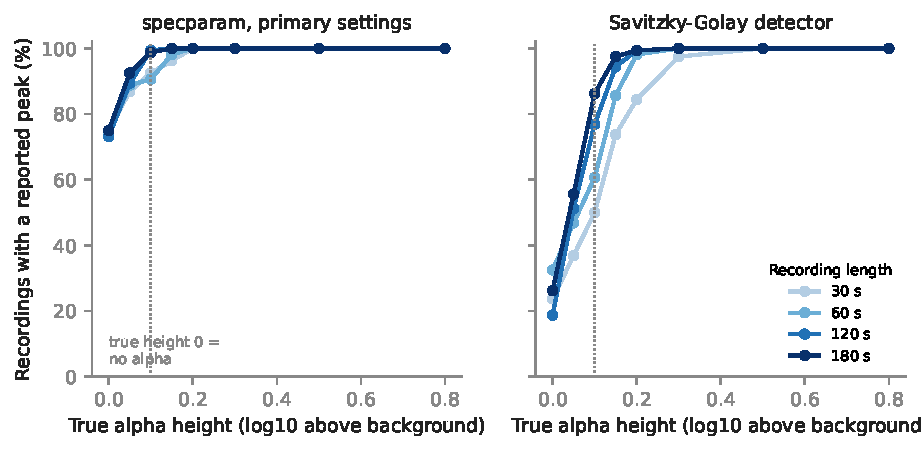
\includegraphics[width=0.9\linewidth]{figures/figS1_detection}
\caption{Share of simulated recordings with a reported alpha peak, by true peak height and
recording length. Left: specparam with the primary settings. Right: the Savitzky--Golay
detector. A true height of 0 means that the recording contains no alpha, so the leftmost
points are false ``present'' rates. The dotted line marks the minimum peak height (0.1).}
\label{fig:simdetect}
\end{figure}

\subsubsection{A threshold on the fitted peak height restores a low false ``present'' rate}

Table~\ref{tab:simrules} compares alternative rules on the same recordings. In no-alpha
recordings, the largest chance peak in the alpha window had a fitted height whose 95th
percentile was 0.25 at 60~s, 0.17 at 120~s and 0.13 at 180~s. A rule that keeps the fit
settings but counts alpha as present only if the fitted height of the tallest peak is at
least 0.25 gave a false ``present'' rate of 4\% at 60~s and 0\% at 120 and 180~s, and
detected 98--100\% of peaks of true height 0.3 or more. Raising specparam's own minimum
height to 0.25 or 0.30 was less effective for short recordings (60\% and 22\% false
``present'' at 60~s). A peak threshold of 3~SD left the false ``present'' rate at 22--24\%.
Using mean instead of median spectra did not help (62--82\%).

No rule separated peaks of true height 0.1--0.2 from chance. With the 0.25 rule, a peak of
height 0.2 was detected in 69\%, 52\% and 34\% of recordings at 60, 120 and 180~s (it is
found less often in longer recordings because its fitted height is overestimated less).
In this dataset, ``alpha present'' can therefore only mean a peak of roughly twice the
background power or more. \TBD{state the rule adopted in the final pre-registration.}

\begin{table}[ht]
\centering
\caption{Alternative presence rules (experiment K; 200 recordings per cell). False
``present'': share of no-alpha recordings with a reported peak at 60 / 120 / 180~s.
Detection: share of recordings with a true peak of the given height in which it is
reported, pooled over lengths (three values are for 60 / 120 / 180~s).}
\label{tab:simrules}
\begin{tabular}{p{0.34\linewidth}p{0.17\linewidth}p{0.17\linewidth}p{0.17\linewidth}}
\toprule
Rule & False ``present'' & Detects 0.2 & Detects 0.3 \\
\midrule
Drafted: minimum height 0.10, threshold 2~SD & 83 / 78 / 74\% & 100\% & 100\% \\
Peak threshold 3~SD & 24 / 23 / 22\% & 94\% & 100\% \\
Minimum height 0.20 & 82 / 29 / 3\% & 100\% & 100\% \\
Minimum height 0.25 & 60 / 3 / 0\% & 86\% & 100\% \\
Minimum height 0.30 & 22 / 0 / 0\% & 54\% & 98\% \\
Minimum height 0.40 & 0 / 0 / 0\% & 7\% & 46\% \\
Fitted height $\geq$ 0.20 & 21 / 0 / 0\% & 88 / 90 / 86\% & 99 / 100 / 100\% \\
Fitted height $\geq$ 0.25 & 4 / 0 / 0\% & 69 / 52 / 34\% & 98 / 100 / 99\% \\
Fitted height $\geq$ 0.30 & 1 / 0 / 0\% & 32 / 11 / 4\% & 89 / 88 / 78\% \\
Mean spectra, minimum height 0.10 & 82 / 80 / 62\% & 100\% & 100\% \\
\bottomrule
\end{tabular}
\end{table}

\subsubsection{Recovery of the exponent, IAF and peak height}

The aperiodic exponent was recovered with a small positive bias of 0.014--0.028 for all
true exponents and lengths. The standard deviation of its error was 0.055 at 60~s, 0.037 at
120~s and 0.030 at 180~s (Figure~\ref{fig:simrecovery}). For a peak of true height 0.3, the
mean absolute error of IAF was 0.36~Hz at 60~s, 0.27~Hz at 120~s and 0.24~Hz at 180~s; for
height 0.5 it was 0.25, 0.19 and 0.19~Hz. Errors above 1~Hz occurred in 1\% or fewer of
recordings for heights of 0.5 or more, but in 3--8\% for height 0.2, where the tallest peak
in the window is sometimes a chance peak. Small peaks were overestimated: for true heights
of 0.2--0.3 the fitted height was 0.02--0.08 too high at 60~s or more. Results at 256~Hz
did not differ from those at 128~Hz.

\begin{figure}[ht]
\centering
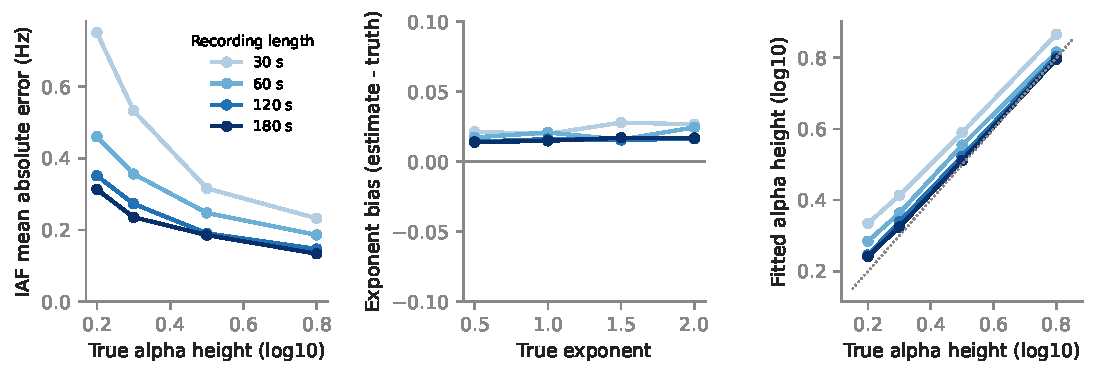
\includegraphics[width=\linewidth]{figures/figS3_recovery}
\caption{Recovery of known parameters in simulated recordings (experiment A, primary
settings). Left: mean absolute error of IAF among detected peaks. Middle: bias of the
aperiodic exponent. Right: fitted against true peak height; the dotted line is identity.}
\label{fig:simrecovery}
\end{figure}

\subsubsection{The simulated cohort}

In the simulated two-site study the planted age slopes were recovered
(Table~\ref{tab:simcohort}). Among participants with planted alpha, 1.1\% were called
absent in each site. Among those planted with no alpha, 43\% and 48\% were called present
under the drafted rule (fewer than in experiment A because this cohort includes a
sensor-noise floor, which lowers the rate; see below). Two tests behaved in a way that
matters for the real analysis. The income odds ratio, planted at 1, had a 90\% interval of
0.72--1.55 with 20 missing peaks among 400 participants, so equivalence within 0.80--1.25
could not be shown although it was true. And alpha power in the first site, planted with
no age effect, had an interval inside the equivalence bounds but did not survive Holm's
correction (adjusted $p = 0.24$).

\begin{table}[ht]
\centering
\caption{Recovery of planted effects in a simulated cohort of 400 participants per site.
Intervals are 95\% for H3 and H4 and 90\% for H5.}
\label{tab:simcohort}
\begin{tabular}{lrrr}
\toprule
 & Planted & Simulated site 1 & Simulated site 2 \\
\midrule
IAF slope, Hz per decade (H3) & $-0.12$ & $-0.144$ [$-0.213$, $-0.076$] & $-0.061$ [$-0.124$, $0.002$] \\
Exponent slope per decade (H4) & $-0.06$ & $-0.062$ [$-0.081$, $-0.044$] & $-0.069$ [$-0.085$, $-0.053$] \\
Alpha power slope, SD per decade (H5) & $0$ & $-0.039$ [$-0.099$, $0.022$] & $0.005$ [$-0.052$, $0.062$] \\
\bottomrule
\end{tabular}
\end{table}

\subsubsection{Conditions under which the method fails}

\emph{Fit-quality floor.} $R^2$ depends on the exponent as well as on fit quality, because
a flat spectrum has little variance for the model to explain. Simulated spectra with
exponent 0.5, fitted without error, fell below $R^2 = 0.90$ in 94\% of 60~s recordings,
58\% of 120~s recordings and 4\% of 180~s recordings. Spectra with exponents of 1.5 or more
never did. The mean absolute fit error was the same for all exponents. A floor on $R^2$
therefore removes flat-spectrum recordings selectively.

\emph{Sensor noise.} A white noise floor as strong as the background at 40~Hz lowered the
fitted exponent by 0.20--0.27; at 25~Hz by 0.35--0.44; at 15~Hz by about 0.6; and at 8~Hz
by about 0.9, where a peak of height 0.2 was found in only 43\% of recordings. Broadband
noise thus makes a spectrum look flatter and can hide a moderate peak. It also lowered the
false ``present'' rate of the drafted rule (to 38\%, 23\%, 10\% and 13\%).

\emph{Filters inside the fit range.} A low-pass filter at 43~Hz raised the fitted exponent
by 0.22, and one at 35~Hz by 0.78.

\emph{Window edges.} A peak centred at exactly 7 or 14~Hz was reported in 95\% and 93\% of
recordings, but its frequency was wrong by more than 1~Hz in about 30\%. Between 7.25 and
13.75~Hz detection was 100\%.

\emph{Intermittent alpha.} When alpha of height 0.6 was present half of the time, its
fitted height fell to 0.34 with median spectra and 0.39 with mean spectra; at 20\% of the
time, to 0.17 and 0.20. With a threshold on fitted height, such recordings can be counted
as having no peak.

\emph{Heavy artefact.} With large bursts in 10\% of the recording, the within-person
outlier rule removed them and estimates were unaffected. With bursts in 30\%, the rule
removed nothing, the exponent was off by $-0.6$ to $-0.7$ and the median $R^2$ was 0.3.

\emph{Line noise.} Line noise at 50~Hz of up to 200~$\mu$V had no effect on detection, IAF
or the exponent, as it lies outside the fit range.

\emph{Aperiodic mode and fit range.} Fitting a knee to spectra without one made the
exponent up to three times more variable, and the 3--30~Hz range raised the false
``present'' rate to 91\%.


\subsection{Sample and data quality}
\TBD{Table 1 from \texttt{results/descriptives.csv}: by site, n, sex, age distribution,
clean seconds, share of epochs kept, EQ, line-noise ratio, number of failed fits, number of
fits below the fit-quality criterion. Figure 1: participant flow (\texttt{fig1\_flow}).
Figure 2: example fits (\texttt{fig2\_examples}).}

\subsection{H1: presence of an alpha peak}
\TBD{Per site: share present with Wilson 95\% CI, exact binomial $p$ against 0.80,
Holm-adjusted $p$, supported or not. Figure 3: presence against the threshold
(\texttt{fig3\_threshold}), with the simulated false ``present'' rate at each threshold
for comparison. Null calibration for each site (\texttt{results/robustness\_summary.csv}).
Source: \texttt{results/confirmatory.csv}.}

\subsection{H2: recording quality, income and missing peaks}
\TBD{Odds ratio per SD of the quality composite with 95\% CI, per site (H2a). Odds ratio
per SD of income rank with 90\% CI, India (H2b), with the number of missing peaks and the
power note. Firth estimates as sensitivity. Figure 4 (\texttt{fig4\_forest}).}

\subsection{H3--H5: age}
\TBD{Slopes per decade with intervals for IAF, exponent and standardised alpha power, per
site; Table 2 with model coefficients; Figure 5 (\texttt{fig5\_age}).}

\subsection{V1: reactivity}
\TBD{Share of participants with stronger alpha eyes-closed than eyes-open, with CI, per
site.}

\subsection{Robustness}
\TBD{Specification curve (Figure 6, \texttt{fig6\_spec\_curve}); leave-one-researcher-out
ranges; raw 7--12~Hz maximum against specparam IAF; $\kappa$ between detectors; models
without the quality covariate; analysis without the 256~Hz recordings.}

\subsection{Descriptive comparison of the two sites (exploratory)}
\TBD{Ages 18--64 only, estimates with confidence intervals and no $p$-values. Any
difference is described as a difference in environment, recording context and data
quality.}


% ---------------------------------------------------------------------------
\section{Discussion}

\subsection{What the simulation study shows}

Spectral parameterization is often presented as the remedy for peak detection that
ignores the aperiodic background. Our simulations show that, at the frequency resolution
and recording lengths of field EEG, it brings a problem of its own. With common settings
and a minimum peak height of 0.1 $\log_{10}$ units, a peak was reported in the alpha range
in about three of four recordings that contained no alpha. A presence rate computed in
this way would be close to 75\% in a sample with no alpha at all. It could not have tested
whether alpha is ``missing'' in anyone. The same caution applies to any study that reads
``a peak was fitted'' as ``an oscillation is present'' without measuring the false-positive
rate of its own pipeline \citep[see also][]{gerster2022,donoghue2022,ostlund2022}.

The simulations also show a way out and its price. A threshold of 0.25 on the fitted
height kept false detections at or below about 5\% for recordings of one minute or more,
and still found practically every peak of true height 0.3 or more. The price is that peaks
of height 0.1--0.2 cannot be told from chance with one to three minutes of data. For this
dataset, the question ``is alpha absent?'' therefore has to be replaced by ``is there an
alpha peak of at least about twice the background power?''. Weak alpha, which is what
\citet{parameshwaran2017} themselves describe as a continuum, lies partly below the
resolution of recordings of this length.

Three further results shape how the real data should be read. First, broadband sensor
noise flattens the fitted exponent and can hide a moderate peak. A recording of lower
quality will then tend to show a flatter spectrum and a missing peak for technical
reasons, which is the mechanism behind our hypothesis H2a and a reason to treat the
exponent as comparable within this dataset only. Second, a fit-quality floor based on
$R^2$ removes flat spectra selectively, which would bias an analysis of how the exponent
changes with age. Third, the planned equivalence test for income (H2b) has little chance
of succeeding with a few dozen missing peaks, even if income has no effect at all, so a
failure of that test must be read as inconclusive.

\subsection{Real-data findings}
\TBD{(1) What the presence rate means for the 2017 claim; if weak or missing alpha
remains, what recording quality explains and what it does not. (2) The age results
compared with \citet{merkin2023}, \citet{cesnaite2023} and \citet{trondle2023}, and with
the raw peak frequencies of \citet{vianney2025}. (3) What the robustness analyses change.}

\subsection{Site differences are not population traits}

India and Tanzania differ in this dataset in ways that have nothing to do with the brains
of the people recorded. Tanzania has 136 electrode layouts and India 10. Different field
teams made the recordings, in different settings. The Indian sample is much younger. How
the 2,000 public participants were chosen from the 7,933 is not documented. Any difference
between the two sites, and any difference between income groups within India, is a
difference between recording contexts, environments and levels of data quality as much as
between groups of people. We report site differences descriptively and draw no conclusion
about innate characteristics of any population. \TBD{add the specific differences observed.}

\subsection{Limitations}

The simulations use stationary Gaussian noise and a spectrum that follows the specparam
model exactly. Real EEG has muscle activity, non-stationary noise and possibly a spectral
knee, so real false-positive rates may differ from the simulated ones in either direction.
Simulation cells have 40 to 200 repetitions, so differences of a few percentage points are
within noise. The built-in filters of the headset are not documented in the public files,
and the files are sampled at 128~Hz although the source paper states 256~Hz. Age is known
only in bins. Income is analysed in one country and falls mostly in two bins. The grouping
of participants by field researcher rests on an undocumented reading of the participant
identifiers. IAF and alpha power are defined only when a peak is detected. The design is
cross-sectional, so age differences are not changes within people. \TBD{limitations that
emerge from the real analysis.}

\subsection{Conclusion}
\TBD{Two or three sentences after the real analysis.}

% ---------------------------------------------------------------------------
\section*{Statements}

\paragraph{Data and code availability.} The EEG data are public: OpenNeuro ds007358,
version 1.0.0, CC0 \citep{openneuro_ds007358}. All code, the pre-registration, the
simulation outputs and the derived tables are in the project repository
(\url{https://github.com/brkh1222-byte/resting-eeg-india-tanzania}). \TBD{archive DOI.}

\paragraph{Ethics.} This is a secondary analysis of de-identified, openly licensed data.
Consent and ethical approvals of the original study are reported by \citet{vianney2025}.

\paragraph{Software.} Python 3.12; MNE-Python 1.10.1 \citep{gramfort2013}; fooof 1.1.1
\citep{donoghue2020}; SciPy 1.15.3 \citep{virtanen2020}; statsmodels 0.14.5
\citep{seabold2010}.

\paragraph{Author contributions.} [AUTHORS --- TBD]

\paragraph{Use of AI tools.} [AI-USE STATEMENT --- TBD]

\paragraph{Competing interests.} \TBD{to be declared by the authors.}

\paragraph{Funding.} \TBD{to be declared by the authors.}


\bibliographystyle{apalike}
\bibliography{references}

\end{document}
